\documentclass{standalone}
\usepackage{tikz}
\begin{document}
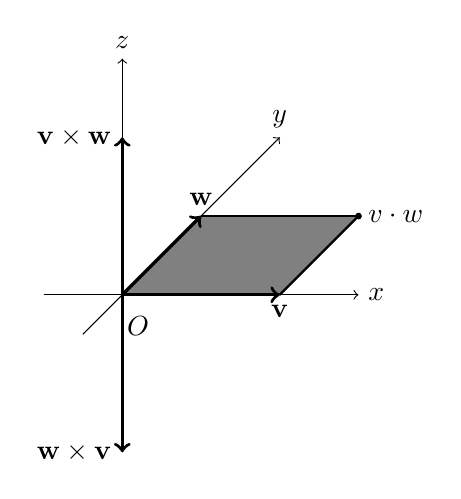
\begin{tikzpicture}[scale=2]
    \coordinate (O) at (0, 0);

    \draw[fill=gray](1.5,0.5)--(1,0)--(O)--(0.5,0.5)--cycle;

    \node[black] at (0.1, -0.2) {$O$};
    \draw[->] (-0.5,0)--(1.5,0) coordinate (x) node[right]{$x$};
    \draw[->] (0,-0.5)--(0,1.5) node[above]{$z$};
    \draw[->] (-0.25, -0.25) -- (1, 1) node[above] {$y$};
    \draw[->,very thick] (O) -- (1, 0) coordinate (v) node[below] {$\mathbf{v}$};
    \draw[->,very thick] (O) -- (0.5, 0.5) coordinate (w) node[above] {$\mathbf{w}$};
    \draw[-,thick] (1,0) -- (1.5, 0.5);
    \draw[-,thick] (0.5, 0.5) -- (1.5, 0.5);
    \filldraw[black](1.5,0.5)circle(0.5pt);
    \node[right]at(1.5,0.5)[right] {$v\cdot w$}; 

    \draw[->,very thick] (O) -- (0, 1) node[left] {$\mathbf{v}\times\mathbf{w}$};
    \draw[->,very thick] (O) -- (0,-1) node[left] {$\mathbf{w}\times\mathbf{v}$};
\end{tikzpicture}
\end{document}